\documentclass[conference]{IEEEtran}
\IEEEoverridecommandlockouts
\usepackage{cite}
\usepackage{amsmath,amssymb,amsfonts}
\usepackage{algorithmic}
\usepackage{algorithm}
\usepackage{graphicx}
\usepackage{textcomp}
\usepackage{xcolor}
\usepackage{booktabs}
\usepackage{url}
\usepackage{balance}
\usepackage{tikz}
\usetikzlibrary{arrows.meta, positioning, shapes.geometric, fit, backgrounds, decorations.pathreplacing, calc}

\begin{document}

\title{NeuroShard: A Decentralized Architecture for Collaborative Large Language Model Training over Heterogeneous Networks}

\author{Anonymous Author(s)}

\maketitle

\begin{abstract}
Recent systems such as OpenDiLoCo, INTELLECT-1, and Photon have demonstrated that large language models (LLMs) can be trained across geographically distributed, weakly connected nodes---but under \emph{curated, permissioned} participant sets: nodes may be slow or fail, yet none is economically motivated to cheat. We present NeuroShard, a protocol extending low-communication decentralized training to \emph{open, permissionless, adversarial} networks of heterogeneous commodity hardware. NeuroShard integrates: (1)~\emph{Quorum-Based Training}, in which speed-matched nodes self-organize into complete pipelines that coordinate across quorums through DiLoCo-style outer-loop aggregation; (2)~\emph{Proof of Neural Work (PoNW)}, an optimistic verification layer building on proof-of-learning, in which signed training proofs are accepted immediately and disputed through stake-weighted challenges resolved by deterministic re-computation; and (3)~\emph{Byzantine-robust aggregation} using coordinate-wise Trimmed Mean and Median with $\sqrt{n}$-weighted contributions. The contribution is the integration of these components into one incentive-aligned protocol, plus an empirical evaluation on an open-source prototype: DiLoCo-style synchronization converges within 3\% of synchronous data parallelism using $50\times$ less communication ($527\times$ with compression), robust aggregation holds validation loss at baseline under 30\% sign-flipping adversaries where undefended averaging diverges, and a three-node deployment survives node failure and rejoin. We analyze security against gradient poisoning, Sybil, free-riding, and proof-spoofing attacks, explicitly engaging known attacks on proof-of-learning verification.
\end{abstract}

\begin{IEEEkeywords}
Decentralized machine learning, distributed training, peer-to-peer networks, Byzantine fault tolerance, consensus protocols, large language models
\end{IEEEkeywords}

\section{Introduction}

The training of frontier large language models (LLMs) such as GPT-4~\cite{openai2023gpt4} is concentrated in a few vertically integrated organizations. This centralization sets alignment policy unilaterally, prices out independent researchers, and leaves the world's edge compute (consumer GPUs, idle CPUs, single-board computers) unused for AI workloads.

A growing body of work shows the \emph{communication} barrier to decentralized training is falling. DiLoCo~\cite{douillard2023diloco} trains independent replicas that synchronize only every $H$ steps; OpenDiLoCo~\cite{jaghouar2024opendiloco} reproduced this across three countries at 1.1B parameters; INTELLECT-1~\cite{jaghouar2024intellect} scaled it to a 10B model trained by 30 independent compute providers with dynamic membership; Photon~\cite{sani2024photon} federates pre-training up to 7B parameters; SWARM parallelism~\cite{ryabinin2023swarm} pipelines models over preemptible, poorly connected devices. These systems establish that low-communication decentralized LLM training is practical---but under a \emph{permissioned} trust model: participants are vetted providers or collaborating institutions, failures are crash-like, and nobody is paid per unit of claimed work. Opening participation to anonymous, economically motivated actors adds three requirements none of these systems addresses jointly: contributions must be \emph{verifiable}, aggregation must be \emph{Byzantine-robust}, and honesty must be \emph{incentive-compatible}.

NeuroShard addresses this gap with an integrated protocol for trustless, incentivized, Byzantine-tolerant collaborative training. A heterogeneous P2P network partitions into speed-matched \emph{quorums}---self-organized complete training pipelines---that train synchronously internally and synchronize across groups periodically via DiLoCo outer-loop updates. On this two-level hierarchy, NeuroShard layers signed work proofs with optimistic challenge-based verification, robust aggregation, and a token economy that makes sustained cheating unprofitable.

We are explicit about the nature of our contribution: the building blocks originate in prior work---DiLoCo~\cite{douillard2023diloco}, robust aggregation estimators~\cite{yin2018byzantine,blanchard2017machine}, proof-of-learning~\cite{jia2021proof}, and optimistic rollups~\cite{kalodner2018arbitrum}. This paper contributes their \emph{composition} into a single protocol for the open adversarial setting, the design decisions that composition forces, and an initial empirical validation.

\smallskip\noindent\textbf{Contributions.}
\begin{itemize}
    \item \textbf{Quorum-Based Training:} nodes self-benchmark into speed tiers and form complete pipelines, letting hardware from data-center GPUs to single-board computers contribute through appropriate modes (Section~\ref{sec:quorum}).
    \item \textbf{Adversarial adaptation of DiLoCo:} cross-quorum synchronization replacing DiLoCo's trusted all-reduce with Byzantine-robust, $\sqrt{n}$-weighted aggregation over gossiped, compressed pseudo-gradients, with an explicit account of what is inherited versus modified (Section~\ref{sec:diloco}).
    \item \textbf{Proof of Neural Work (PoNW):} an optimistic verification layer building on proof-of-learning~\cite{jia2021proof} and engaging its known spoofing attacks~\cite{zhang2022adversarial,fang2023proof}: proofs commit to deterministic data shards and chained model states; challenges are resolved by exact re-computation rather than statistical plausibility (Section~\ref{sec:ponw}).
    \item \textbf{Prototype and evaluation:} an open-source Python prototype (${\sim}48$k lines plus 20k-line test suite) and experiments measuring (i) the convergence--communication trade-off vs.\ synchronous data parallelism, (ii) robust aggregation under attack at 10--40\% adversarial fractions, (iii) compression fidelity, (iv) PoNW overheads, and (v) fault tolerance under churn (Section~\ref{sec:eval}).
\end{itemize}

\section{Related Work}

\subsection{Federated and Distributed Learning}

Federated Learning (FL)~\cite{mcmahan2017communication} trains across decentralized devices, keeping data local and aggregating updates centrally. FedAvg successors~\cite{karimireddy2020scaffold} address statistical heterogeneity but retain a trusted aggregator. Later designs relax this: Swarm Learning~\cite{warnat2021swarm} replaces the server with blockchain-coordinated peer aggregation, and fully decentralized FL over gossip topologies is well studied~\cite{kairouz2021advances}. NeuroShard follows this decentralized line but additionally assumes actively malicious, per-contribution-paid participants. AllReduce data parallelism~\cite{goyal2017accurate} needs synchronous communication every step, infeasible over wide-area links; local SGD~\cite{stich2019local} reduces frequency but assumes homogeneous, honest participants.

\subsection{Pipeline Parallelism over Unreliable Nodes}

GPipe~\cite{huang2019gpipe} and PipeDream partition models by layers within data centers. SWARM parallelism~\cite{ryabinin2023swarm} extends pipelining to preemptible, heterogeneous nodes with stochastic rewiring, training a 1B-parameter model on sub-200\,Mb/s links. Petals~\cite{borzunov2023petals} serves \emph{inference} over volunteer nodes. NeuroShard's quorums are speed-matched pipelines in this tradition; the difference is the verification and incentive layer wrapped around them.

\subsection{Decentralized LLM Training at Scale}
\label{sec:related-decentralized}

Closest to our setting are the DiLoCo-lineage systems. DiLoCo~\cite{douillard2023diloco} introduced the inner/outer optimization split with Nesterov outer momentum. OpenDiLoCo~\cite{jaghouar2024opendiloco} provides an open implementation on Hivemind~\cite{ryabinin2020hivemind}, demonstrating intercontinental training at 90--95\% utilization. INTELLECT-1~\cite{jaghouar2024intellect} trained a 10B model over 1T tokens across three continents with 30 providers joining and leaving, using PRIME's ElasticDeviceMesh for fault tolerance and int8 pseudo-gradient all-reduce for a reported $400\times$ bandwidth reduction. Photon~\cite{sani2024photon} (behind the federated ``FlowerLLM'' models) trains up to 7B-parameter LLMs cross-silo with $64$--$512\times$ less communication. These systems demonstrate scale, fault tolerance, and communication efficiency---but all assume a \emph{closed set of known participants}: none verifies that a submitted pseudo-gradient reflects real computation, defends aggregation against coordinated manipulation, or meters rewards. NeuroShard targets precisely this open-membership regime; conversely, we inherit our communication efficiency from their shared foundation and do not claim it as novel. Bittensor~\cite{bittensor} runs an open incentive market but scores model \emph{outputs} rather than coordinating gradient-level co-training; Gensyn~\cite{gensyn} targets verifiable ML compute without a complete training protocol.

\subsection{Byzantine-Robust Aggregation}

Blanchard et al.~\cite{blanchard2017machine} introduced Krum and Multi-Krum for Byzantine-tolerant gradient descent. Yin et al.~\cite{yin2018byzantine} proposed and analyzed \emph{coordinate-wise median} and \emph{coordinate-wise trimmed mean}, proving order-optimal statistical rates; these two estimators are the defaults in NeuroShard's cohort aggregation, and our tolerance target derives from their breakdown analysis (Section~\ref{sec:byzantine}). Robust aggregation under non-i.i.d.\ data and adaptive attacks remains an active area~\cite{kairouz2021advances}.

\subsection{Verifiable Training and Proof-of-Learning}

Jia et al.~\cite{jia2021proof} introduced proof-of-learning (PoL): a prover logs training checkpoints so a verifier can replay segments and confirm compute expenditure, explicitly motivated by distributed training across untrusted workers. Subsequent attacks showed PoL verification is fragile: Zhang et al.~\cite{zhang2022adversarial} synthesize valid-looking proofs at a fraction of honest cost via adversarial-example-style optimization, and Fang et al.~\cite{fang2023proof} demonstrate cheaper, reproducible spoofs, arguing robust PoL verification reduces to open problems in learning theory. PoNW is a blockchain-anchored descendant of PoL and is therefore designed \emph{assuming} statistical verification can be gamed (Section~\ref{sec:ponw-spoofing}). TOPLOC~\cite{ong2025toploc} provides locality-sensitive activation hashing robust to hardware non-determinism---used in INTELLECT-2~\cite{primeintellect2025intellect2} for verifiable RL rollouts---and is a natural upgrade path for PoNW's commitments.

\section{System Architecture}
\label{sec:architecture}

\subsection{Network Layer}

NeuroShard operates on a structured P2P overlay built on a Kademlia DHT~\cite{maymounkov2002kademlia}. Nodes bootstrap via trackers, then rely on decentralized DHT discovery with gossip redundancy; each advertises its memory, measured speed, bandwidth, held layers, quorum membership, stake, and reputation. The stack has four planes: \emph{network} (DHT, gossip, trackers), \emph{node} (self-benchmarking, dynamic layer pool, contribution modes), \emph{training} (quorum formation, pipeline execution, DiLoCo outer sync), and \emph{consensus} (PoNW proofs chained into epochs driving the NEURO ledger).

\subsection{Speed Tiers and Contribution Modes}
\label{sec:tiers}

Upon joining---and periodically thereafter---every node self-benchmarks by measuring forward-pass latency per transformer layer on its own hardware. The \emph{measured latency}, not the device model, determines tier membership (Table~\ref{tab:tiers}); the hardware column is illustrative only. Because classification re-runs at intervals and on quorum renewal, membership is fluid: a node whose effective throughput changes (throttling, contention, upgrades) migrates automatically. Thresholds are protocol configuration, not architectural constants, and the classifier could equally consume a continuous throughput metric (tokens/s per layer); we adopt discrete tiers because quorum formation needs an equivalence relation for speed matching (adjacent tiers are compatible, e.g., T2 pairs with T1--T3), and coarse buckets are robust to benchmark noise.

\begin{table}[t]
\caption{Speed tiers (config-defined thresholds; hardware illustrative)}
\label{tab:tiers}
\centering
\begin{tabular}{@{}llll@{}}
\toprule
\textbf{Tier} & \textbf{Latency/Layer} & \textbf{Typical hardware} & \textbf{Role} \\
\midrule
T1 & $<$10\,ms & H100, A100 & Pipeline leader \\
T2 & 10--50\,ms & RTX 4090/3090 & Pipeline member \\
T3 & 50--200\,ms & RTX 3060, fast CPU & Pipeline member \\
T4 & 200--1000\,ms & Older GPU, CPU & Pipeline/async \\
T5 & $>$1000\,ms & Raspberry Pi & Async only \\
\bottomrule
\end{tabular}
\end{table}

Nodes operate in one of six modes based on tier and network needs: \emph{Pipeline} (real-time quorum member), \emph{Async} (offline training, periodic gradient submission), \emph{Data} (serving training shards), \emph{Verify} (challenging PoNW proofs), \emph{Inference}, or \emph{Idle}.

\subsection{Model Architecture and Capacity Scaling}
\label{sec:model}

NeuroShard trains NeuroLLM, a decoder-only transformer whose components are chosen for decentralized operation. RMSNorm~\cite{zhang2019root} avoids LayerNorm's mean-centering, improving numerical stability when layer shards train on heterogeneous float stacks. Rotary Position Embeddings~\cite{su2021roformer} encode position in attention rather than learned tables, so pipeline stages share no positional state and depth can change without invalidating embeddings. Grouped Query Attention~\cite{ainslie2023gqa} shrinks KV projections, cutting both consumer-GPU memory and the activation volume streamed between stages. SwiGLU~\cite{shazeer2020glu} follows best practice for quality per parameter; embeddings are tied to save memory on nodes hosting the frequently replicated first/last layers; sparse Mixture-of-Experts layers (top-2 routing) are supported for future width scaling, as experts parallelize naturally across nodes.

The architecture is not fixed: the network re-derives a parameter budget from aggregate capacity. With total advertised memory $M_{\text{total}} = \sum_i M_i$, utilization factor $u$ (default 0.6), training-state footprint $b$ per parameter (16 bytes: fp32 weights, gradients, Adam moments), and target replication $R$,
\begin{equation}
P_{\max} = \frac{u \cdot M_{\text{total}}}{b \cdot R}. \label{eq:budget}
\end{equation}
A single 2\,GB node yields ${\sim}50$M parameters; 1000 nodes averaging 8\,GB support order-$10^{11}$ parameters at $R{=}3$ \emph{by memory budget alone}---a capacity bound, not a demonstrated run, and per-node bandwidth binds well before memory (Section~\ref{sec:limitations}). Given a budget, width and depth follow a width-biased allocation (hidden dimension ${\propto}P^{0.6}$, depth ${\propto}P^{0.4}$ within each phase band). This is an engineering heuristic motivated by the observation that width should grow faster than depth~\cite{kaplan2020scaling,hoffmann2022training}; the exponents are not prescribed by scaling-law theory, and the registry migrates architectures only when the budget crosses hysteresis thresholds. Layers are distributed via a DHT-based \emph{Dynamic Layer Pool} with replication $R \geq 2$; scarcity incentives reward hosting under-replicated layers:
\begin{equation}
M_{\text{scarcity}} = 1 + 0.5 \times \frac{R_{\text{target}} - R_{\text{actual}}}{R_{\text{target}}}. \label{eq:scarcity}
\end{equation}

\section{Quorum-Based Training}
\label{sec:quorum}

\subsection{Quorum Formation and Pipeline Execution}

A \emph{quorum} is a self-organized group of speed-compatible nodes that collectively hold all model layers, forming a complete training pipeline. An initiating node queries the DHT for layer holders in compatible tiers; a greedy selection maximizes layer coverage while minimizing inter-node latency; on complete coverage the initiator proposes the quorum, which registers in the DHT upon unanimous acceptance (otherwise the node falls back to asynchronous mode). Quorums are \emph{complete} (all layers covered), \emph{speed-matched}, \emph{self-sufficient} (no external coordinator), and \emph{temporary} (roughly one-hour sessions, renewed at 80\% if health checks pass). Within a quorum, roles follow layer assignment: the \textbf{initiator} (embedding) fetches a batch and starts the forward pass; \textbf{processors} forward activations; the \textbf{finisher} (LM head) computes the loss and starts the backward pass. Each node applies local AdamW to its layers, accumulating updates toward the next cross-quorum synchronization.

\subsection{Multi-Speed Quorums and Stragglers}
\label{sec:multispeed}

The network naturally forms quorums at different throughputs (fast T1--T2, medium T2--T3, slow T3--T4); each is internally synchronous but asynchronous relative to others. T5 devices contribute via async mode: they download weights, train locally, and submit pseudo-gradients discounted by freshness decay. Because quorums differ in throughput, demanding an identical inner-step count $H$ of all quorums would stall fast ones at sync barriers. The outer sync is therefore a \emph{time-window} rendezvous: each quorum contributes whatever inner progress it completed within the window, weighted by actual batch counts via the $\sqrt{n}$ scheme of Section~\ref{sec:sqrtn} ($H{=}500$ is the reference cadence for a mid-tier quorum). This mirrors the adaptive local parallelism of Photon~\cite{sani2024photon}; systematic per-tier $H$ selection is future work.

\subsection{Gradient Compression}
\label{sec:compression}

To reduce bandwidth within and across quorums, NeuroShard compresses pseudo-gradients with a standard pipeline drawn from the communication-efficient training literature: Top-$K$ sparsification (keep the largest-magnitude coordinates)~\cite{lin2018deep}, 8-bit quantization of retained values~\cite{alistarh2017qsgd}, entropy coding (zlib), and \emph{error feedback} that accumulates the discarded residual into the next round's update to preserve convergence~\cite{karimireddy2019error}. Section~\ref{sec:eval-compression} reports measured compression ratios and fidelity on real pseudo-gradients; at the default $K{=}10\%$ the pipeline yields ${\sim}11\times$ compression with cosine fidelity 0.58 to the uncompressed delta, with error feedback re-injecting the residual over subsequent rounds (Fig.~\ref{fig:convergence}).

\section{Cross-Quorum Synchronization}
\label{sec:diloco}

\subsection{Outer-Loop Protocol: What Is Inherited, What Is New}
\label{sec:outer}

Communication operates at two levels: the \emph{inner loop} is synchronous pipeline training within each quorum with zero cross-quorum traffic; after $H$ inner steps (reference $H{=}500$), the \emph{outer loop} synchronizes each layer across quorums. At each outer point, all holders of a layer form a \emph{Layer Cohort} and execute:
\begin{enumerate}
    \item Each node computes its pseudo-gradient $\Delta w = w_H - w_0$ over the inner loop.
    \item Pseudo-gradients are compressed (Section~\ref{sec:compression}) and exchanged within the cohort via gossip ($k{=}3$ random peers).
    \item The cohort aggregate is computed with Byzantine-robust aggregation (Section~\ref{sec:byzantine}).
    \item The outer optimizer applies the aggregate with Nesterov momentum:
\end{enumerate}
\begin{align}
m_{t+1} &= \beta \cdot m_t + \Delta w_{\text{agg}}, \label{eq:momentum} \\
w_{t+1} &= w_t + \eta_{\text{outer}} \cdot (\beta \cdot m_{t+1} + \Delta w_{\text{agg}}), \label{eq:nesterov}
\end{align}
with $\beta = 0.9$, $\eta_{\text{outer}} = 0.7$.

Steps 1 and 4---the inner/outer split, pseudo-gradient definition, Nesterov outer optimizer, and the hyperparameters $(H, \eta_{\text{outer}}, \beta)$---are adopted \emph{unchanged} from DiLoCo~\cite{douillard2023diloco} as validated by OpenDiLoCo~\cite{jaghouar2024opendiloco}. NeuroShard's modifications are confined to steps 2 and 3: (i) the trusted all-reduce over a known worker set is replaced by gossip within DHT-discovered layer cohorts, since global membership is unknown; (ii) plain averaging is replaced by validated, Byzantine-robust, $\sqrt{n}$-weighted aggregation, since cohort members are untrusted; and (iii) updates are compressed with error feedback, since cohort links are consumer-grade. Each proof of cohort participation is additionally committed to the PoNW chain (Section~\ref{sec:ponw}).

\subsection{Bandwidth Accounting}
\label{sec:bandwidth}

We separate the two factors in NeuroShard's communication reduction to avoid over-claiming. Synchronizing every $H$ steps instead of every step is DiLoCo's contribution, not ours: at $H{=}500$, a worker transmits $500\times$ fewer updates than AllReduce. The second factor is payload compression (${\sim}11\times$ at defaults, Section~\ref{sec:eval-compression}). The product is consistent with INTELLECT-1's $400\times$ with int8 all-reduce~\cite{jaghouar2024intellect} and Photon's $64$--$512\times$~\cite{sani2024photon}; our own measurement (Section~\ref{sec:eval-convergence}) shows $527\times$ per-worker byte reduction at $H{=}50$ with compression (12\% loss penalty at the 500-step horizon), or $50\times$ uncompressed within 3\% of synchronous loss. A synchronous baseline could itself compress gradients, so the honest comparison is the measured loss-versus-bytes frontier of Fig.~\ref{fig:convergence}(b).

\begin{figure}[t]
\centering
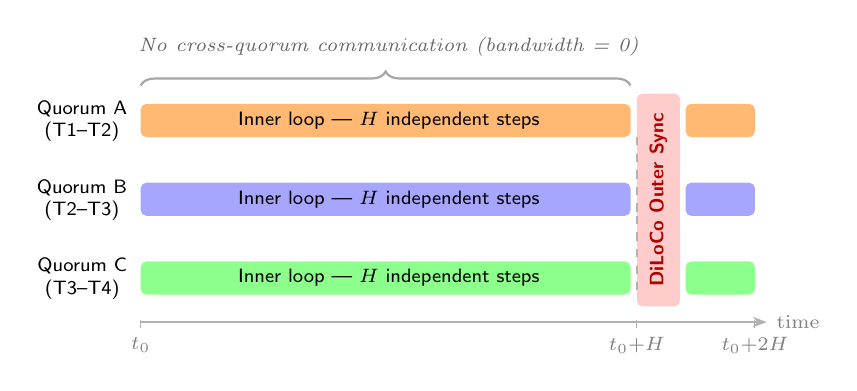
\begin{tikzpicture}[
  font=\scriptsize\sffamily,
  every node/.style={align=center}
]

%% Parameters
\def\W{7.8}   % total timeline width
\def\H{0.42}  % bar height
\def\sync{6.3}% x-position of outer sync

%% ---- Row labels ----
\node[anchor=east, font=\scriptsize\sffamily] at (-0.05, 2.1) {Quorum A\\(T1--T2)};
\node[anchor=east, font=\scriptsize\sffamily] at (-0.05, 1.1) {Quorum B\\(T2--T3)};
\node[anchor=east, font=\scriptsize\sffamily] at (-0.05, 0.1) {Quorum C\\(T3--T4)};

%% ---- Inner-loop bars ----
\fill[orange!55, rounded corners=2pt]
  (0, 1.9) rectangle (\sync-0.08, 1.9+\H);
\node[font=\scriptsize\sffamily] at (\sync/2, 1.9+\H/2)
  {Inner loop — $H$ independent steps};

\fill[blue!35, rounded corners=2pt]
  (0, 0.9) rectangle (\sync-0.08, 0.9+\H);
\node[font=\scriptsize\sffamily] at (\sync/2, 0.9+\H/2)
  {Inner loop — $H$ independent steps};

\fill[green!45, rounded corners=2pt]
  (0,-0.1) rectangle (\sync-0.08,-0.1+\H);
\node[font=\scriptsize\sffamily] at (\sync/2,-0.1+\H/2)
  {Inner loop — $H$ independent steps};

%% ---- Outer sync column ----
\fill[red!20, rounded corners=2pt]
  (\sync, -0.25) rectangle (\sync+0.55, 2.45);
\node[rotate=90, font=\scriptsize\bfseries\sffamily, text=red!70!black]
  at (\sync+0.275, 1.1) {DiLoCo Outer Sync};

%% ---- Post-sync bars ----
\fill[orange!55, rounded corners=2pt]
  (\sync+0.62, 1.9) rectangle (\W, 1.9+\H);
\fill[blue!35,  rounded corners=2pt]
  (\sync+0.62, 0.9) rectangle (\W, 0.9+\H);
\fill[green!45, rounded corners=2pt]
  (\sync+0.62,-0.1) rectangle (\W,-0.1+\H);

%% ---- Vertical dashed convergence lines ----
\draw[dashed, gray!60, thick]
  (\sync, 1.9) -- (\sync, 0.9);
\draw[dashed, gray!60, thick]
  (\sync, 0.9) -- (\sync,-0.1);

%% ---- Brace + label ----
\draw[decorate,
      decoration={brace, amplitude=5pt, raise=3pt},
      thick, gray!70]
  (0, 2.45) -- (\sync-0.08, 2.45);
\node[above=10pt, font=\scriptsize\itshape, gray!80!black]
  at (\sync/2, 2.45)
  {No cross-quorum communication (bandwidth = 0)};

%% ---- Timeline axis ----
\draw[-{Stealth[length=5pt]}, thick, gray!60]
  (0,-0.45) -- (\W+0.15,-0.45);
\node[right, font=\scriptsize, gray] at (\W+0.15,-0.45) {time};

%% ---- Tick marks ----
\foreach \x in {0, \sync, \W}{
  \draw[gray!60] (\x,-0.42) -- (\x,-0.52);
}
\node[below, font=\scriptsize, gray] at (0,-0.52)     {$t_0$};
\node[below, font=\scriptsize, gray] at (\sync,-0.52) {$t_0{+}H$};
\node[below, font=\scriptsize, gray] at (\W,-0.52)    {$t_0{+}2H$};

\end{tikzpicture}
\caption{Two-level synchronization: quorums train independently for a sync window (reference $H{=}500$) with zero cross-quorum bandwidth; outer syncs aggregate pseudo-gradients per Layer Cohort robustly.}
\label{fig:diloco-timeline}
\end{figure}

\section{Proof of Neural Work}
\label{sec:ponw}

\subsection{Design Rationale and Relation to Proof-of-Learning}

In an open network, nodes must prove they performed genuine training to receive rewards. PoNW descends from \emph{proof-of-learning}~\cite{jia2021proof}, which established that SGD's stochastic trajectory can evidence expended compute, motivated by exactly our setting---distributed training across untrusted workers. PoNW differs from classic PoL in three ways dictated by the P2P deployment: proofs are (i) \emph{cheap commitments} (hashes of model state, data shard, and gradient statistics) rather than full checkpoint logs; (ii) \emph{signed and chained} into a public epoch ledger; and (iii) verified \emph{optimistically}---accepted immediately, disputed by staked challenges---borrowing the fraud-proof pattern of optimistic rollups~\cite{kalodner2018arbitrum} to keep verification off the critical path.

\subsection{Optimistic Verification Protocol}

After a training round, a node publishes an ECDSA-signed (secp256k1) proof to the DHT containing its identity, work metrics (batches, tokens, layers), model state hashes $h_{\text{start}} \neq h_{\text{end}}$, a gradient commitment $c = \text{SHA-256}(h_{\text{model}} \,\|\, h_{\text{data}} \,\|\, \|\nabla\|_2 \,\|\, \mathcal{L})$, and an epoch identifier. For a 10-minute window, any staked node may challenge by posting a bond; unchallenged proofs finalize. On challenge, the prover supplies the deterministic shard reference and claimed step count, and the challenger \emph{re-executes the claimed steps} on the same shard, comparing outcomes against the commitments. Proven fraud slashes $2\times$ the prover's stake; a failed challenge forfeits the challenger's bond.

\subsection{Chained Proof Structure}

Proofs aggregate into per-epoch Merkle trees linked by hash ($\text{epoch}_i.\text{prev\_hash} = \text{Hash}(\text{epoch}_{i-1})$), with continuity constraints $\text{epoch}_i.\text{model\_start} = \text{epoch}_{i-1}.\text{model\_end}$ and stake-weighted proposer signatures. Chaining matters beyond auditability: each node's claimed step counter and state hash must extend its own previous commitments, so a node cannot retroactively inflate \emph{how many} rounds it executed---a claim of $B$ batches must be consistent with wall-clock epoch spacing, the per-hour proof cap, and physical rate ceilings (no sustained rate above 100 batches/s is accepted), closing the claimed-rounds inflation channel.

\subsection{Adaptive Verification Rate}
\label{sec:adaptive}

Beyond voluntary challenges, verifier-mode nodes spot-check a fraction of proofs by re-computation. The spot-check probability decreases with network size $N$ to bound aggregate verification cost: $P_{\text{verify}} = 1.0$ for $N{<}20$, $0.5$ for $N{<}100$, $0.2$ for $N{<}500$, and $0.05$ beyond. Even at the 5\% floor, a node submitting 100 fraudulent proofs escapes all checks with probability $0.95^{100} \approx 0.6\%$; detecting any single fraud forfeits twice the stake, dominating the accumulated rewards (Section~\ref{sec:game}).

\subsection{Game-Theoretic Analysis}
\label{sec:game}

Let $R$ be the per-proof reward, $S$ the prover's stake, $p$ the probability a fraudulent proof is examined (spot-check or challenge), and $q$ the probability examination detects fraud. One fraudulent proof has expected value
\begin{equation}
\mathbb{E}[\text{fraud}] = (1 - pq) \cdot R - pq \cdot 2S, \label{eq:ev}
\end{equation}
negative for any non-trivial $pq$ since $S \gg R$ (stakes are $10^2$--$10^3\times$ the per-proof reward). The load-bearing assumption is $q \approx 1$: \emph{examination must actually detect fraud}. This is exactly what PoL spoofing attacks undermine~\cite{zhang2022adversarial,fang2023proof}, so we treat it explicitly rather than asserting it.

\subsection{Proof Spoofing: Attacks and Mitigations}
\label{sec:ponw-spoofing}

Zhang et al.~\cite{zhang2022adversarial} and Fang et al.~\cite{fang2023proof} construct checkpoint sequences that pass PoL's \emph{statistical} verification (reproduction-error thresholds over sampled segments) at a fraction of honest cost. Three properties of PoNW change this attack surface. \textbf{(a)~Exact re-computation on committed data:} PoL accepts replayed segments landing \emph{near} claimed checkpoints, and the spoofs exploit that tolerance; a PoNW challenge re-executes the claimed steps from $h_{\text{start}}$ on a \emph{deterministic, committed shard} ($\text{shard} = \text{Hash}(\text{node\_id}) \bmod S$, pinned ordering, seeds, hyperparameters) and requires commitment equality---removing the spoofer's freedom to choose data points or interpolate trajectories. \textbf{(b)~Bounded value per proof:} PoL protects a one-shot, high-value claim (model ownership); PoNW proofs each gate a micro-reward capped per proof and per day, so an attacker must spoof repeatedly against i.i.d.\ spot-checks (Section~\ref{sec:adaptive}), compounding detection probability. \textbf{(c)~Damage bounding independent of verification:} even an undetected free-rider's gradient influence is trimmed by robust aggregation (Section~\ref{sec:byzantine})---verification protects the \emph{reward ledger}, robust aggregation protects the \emph{model}. \textbf{Residual risk:} exact-equality replay assumes reproducible arithmetic; cross-hardware floating-point non-determinism forces some tolerance, partially reopening the statistical-verification gap. Locality-sensitive activation commitments such as TOPLOC~\cite{ong2025toploc}---robust to hardware non-determinism and already deployed for decentralized RL in INTELLECT-2~\cite{primeintellect2025intellect2}---are the planned replacement for PoNW's hash commitments (Section~\ref{sec:limitations}).

\section{Byzantine-Robust Gradient Aggregation}
\label{sec:byzantine}

\subsection{Threat Model and the Origin of $f < 0.3N$}

We assume up to $f$ adversarial nodes per Layer Cohort of size $N$, submitting arbitrary vectors, possibly coordinated, but unable to forge ECDSA signatures. The protocol targets $f < 0.3N$---a bound that is not arbitrary: trimmed mean with trim fraction $\beta$ tolerates adversarial fractions $\alpha \le \beta$ with order-optimal error~\cite{yin2018byzantine} (NeuroShard trims $\beta{=}0.3$ per tail), coordinate-wise median tolerates up to $1/2$~\cite{yin2018byzantine}, and classical BFT agreement requires $f < N/3$. We adopt $0.3$---just inside $1/3$---so both the estimators and stake-weighted consensus operate within their validity regions; breakdown at and beyond this point is measured in Section~\ref{sec:eval-byzantine}.

\subsection{Aggregation Methods}

NeuroShard implements three estimators, selectable per cohort. \textbf{Coordinate-wise Trimmed Mean} and \textbf{Median} are due to Yin et al.~\cite{yin2018byzantine}, who established their statistical optimality for Byzantine distributed learning:
\begin{equation}
\bar{g}_j = \frac{1}{N - 2\lfloor \beta N \rfloor} \sum_{i \in \mathcal{S}_j} g_{i,j},
\qquad
\bar{g}_j = \operatorname{median}_i(g_{i,j}), \label{eq:robust}
\end{equation}
where $\mathcal{S}_j$ excludes the top and bottom $\beta$ fraction per coordinate. \textbf{Multi-Krum}~\cite{blanchard2017machine} averages the $m$ vectors with smallest summed nearest-neighbor distances, giving whole-vector robustness to coordinated attacks. Before aggregation, submissions pass validation screens (cosine similarity to a local reference, magnitude/variance-ratio bounds, $3\sigma$ outlier rejection).

\subsection{$\sqrt{n}$-Weighted Contributions}
\label{sec:sqrtn}

To prevent high-throughput nodes from dominating consensus on the update direction, contributions are weighted by the square root of batches processed:
\begin{equation}
w_i = \sqrt{B_i} \times f_i, \label{eq:sqrtn}
\end{equation}
where $f_i$ is a freshness decay factor. A node processing 100 batches has $10\times$ (not $100\times$) the influence of a single-batch node. We stress the scope of this concavity: it applies to \emph{aggregation influence} only. Economic rewards remain \emph{linear} in batches processed (Section~\ref{sec:incentives}), so capable nodes are not discouraged from contributing capacity; what saturates is their unilateral control over the model's trajectory, which is precisely the Sybil-relevant quantity.

\section{Security Analysis}
\label{sec:security}

\subsection{Attack Surface}

Table~\ref{tab:attacks} maps attacks to defenses. The catalog draws on the FL threat survey of Kairouz et al.~\cite{kairouz2021advances}, the NIST adversarial-ML taxonomy~\cite{vassilev2024adversarial}, the Byzantine-ML literature~\cite{blanchard2017machine,yin2018byzantine}, and the PoL attack line~\cite{zhang2022adversarial,fang2023proof}; it is scoped to training-time attacks on protocol integrity (inference-time attacks and data privacy are out of scope).

\begin{table}[t]
\caption{Attack Types and Defenses}
\label{tab:attacks}
\centering
\small
\begin{tabular}{@{}p{1.5cm}p{2.0cm}p{2.0cm}p{1.5cm}@{}}
\toprule
\textbf{Attack} & \textbf{Detection} & \textbf{Defense} & \textbf{Penalty} \\
\midrule
Free-riding & PoNW spot-checks & Commitment re-execution & $2\times$ slash \\
Gradient poison & Magnitude \& distribution screens & Robust aggregation & Gradient rejected \\
Proof spoofing & Exact replay on pinned shard & Determinism + bounded reward/proof & $2\times$ slash \\
Sybil & Stake analysis & Min.\ stake; $\sqrt{n}$ influence & Clones slashed \\
Quorum collusion & Cross-quorum audit & Random verification & Quorum dissolved \\
Replay & Timestamp \& nonce checks & 5-min freshness window & Proof rejected \\
\bottomrule
\end{tabular}
\end{table}

\subsection{Poisoning, Sybil, and Free-Riding Defenses}

Against \emph{poisoning}, defense is layered: statistical screening rejects gradients deviating more than $3\sigma$ from cohort statistics or failing magnitude/cosine bounds; robust aggregation~\eqref{eq:robust} bounds the influence of survivors; and loss-based verification confirms the aggregate reduces validation loss. One honest caveat from the poisoning literature: attacks crafted to sit \emph{inside} statistical norms (e.g., small-magnitude backdoors) evade screens; trimmed estimators bound their per-round influence to that of any honest minority (quantified in Section~\ref{sec:eval-byzantine}), but certified guarantees under non-i.i.d.\ data remain open. Against \emph{Sybil} attacks, minimum stakes make clone armies capital-intensive, and $\sqrt{n}$ weighting makes them unrewarding: splitting $B$ batches across $k$ identities yields influence $k\sqrt{B/k} = \sqrt{kB}$---sublinear gain purchased with $k$ stakes---while IP/hardware fingerprinting flags suspicious clusters for prioritized verification. Against \emph{free-riding}, each proof's commitment $c$ binds model state, deterministic data shard, and gradient statistics; deterministic shard assignment lets any verifier fetch the identical batch sequence, removing prover control over verification inputs.

\section{Incentive Mechanism}
\label{sec:incentives}

A node's reward per proof epoch is
\begin{equation}
R = R_{\text{base}} \times L \times B \times M_{\text{role}} \times M_{\text{scarcity}} \times M_{\text{stake}}, \label{eq:reward}
\end{equation}
with $R_{\text{base}} = 0.0005$~NEURO per batch per layer, $L$ layers held, $B$ batches, additive role bonuses $M_{\text{role}}$ (processor 1.0; $+0.2$ initiator; $+0.3$ finisher; $+0.1$ actively training), $M_{\text{scarcity}}$ from~\eqref{eq:scarcity}, and
\begin{equation}
M_{\text{stake}} = 1 + 0.1 \cdot \log_2\!\left(1 + \frac{S}{1000}\right). \label{eq:stake}
\end{equation}

Two diminishing-returns curves appear here with distinct targets. The \emph{stake} multiplier~\eqref{eq:stake} is deliberately logarithmic (100{,}000 staked NEURO yields $1.66\times$, vs.\ $11\times$ under a linear rule) to prevent wealth compounding into control. The \emph{work} term is linear: $10\times$ the batches earns $10\times$ the base reward; only aggregation \emph{influence} is concave ($\sqrt{n}$, Section~\ref{sec:sqrtn}). This split answers a natural concern---the network does need very capable nodes, and capping their \emph{earnings} would drive them away---so NeuroShard caps unilateral \emph{steering power} instead, with per-proof/per-day mint ceilings bounding ledger abuse rather than honest throughput. A 5\% burn on transfers and inference payments, plus burning half of slashed stakes, provides deflationary pressure.

\section{Evaluation}
\label{sec:eval}

We evaluate a full prototype: ${\sim}48$k lines of Python implementing the DHT, gossip, quorum formation, DiLoCo trainer, robust aggregation, compression, PoNW verifier, and ledger, plus a ${\sim}20$k-line test suite. Experiments run the \emph{actual implementation classes} (not re-implementations) on a 4-vCPU host; models are small NeuroLLM configurations trained as byte-level LMs on TinyShakespeare. The goal is protocol validation---does the composed system behave as designed under attack, compression, and churn?---not language-modeling quality; large-scale GPU deployment is future work. All harnesses and raw results ship with the code.

\subsection{Convergence versus Communication}
\label{sec:eval-convergence}

\begin{figure*}[t]
\centering
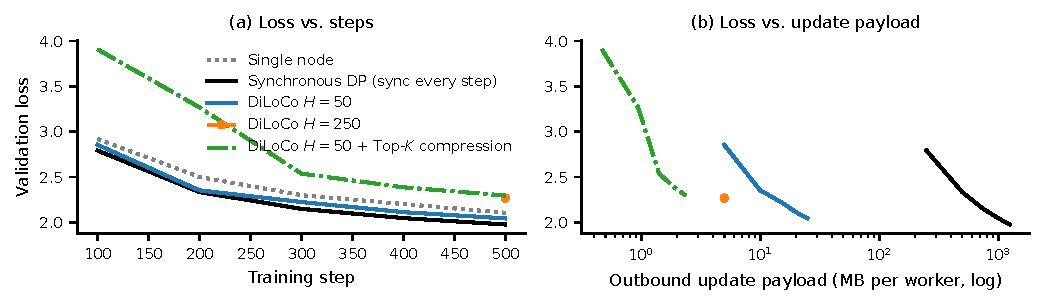
\includegraphics[width=\textwidth]{figures/eval_convergence.pdf}
\caption{Convergence--communication trade-off (0.62M-parameter NeuroLLM, byte-level TinyShakespeare, 3 workers, disjoint shards, 500 steps). (a)~DiLoCo outer sync ($\eta_{\text{outer}}{=}0.7$, $\beta{=}0.9$) tracks synchronous data parallelism per step. (b)~Same runs vs.\ cumulative bytes per worker: $50\times$ ($H{=}50$) to $250\times$ ($H{=}250$) fewer bytes, $527\times$ with compression.}
\label{fig:convergence}
\end{figure*}

Three workers with disjoint shards train a 0.62M-parameter NeuroLLM for 500 steps under: (i)~synchronous data parallelism (gradients averaged every step); (ii)~DiLoCo with $H \in \{50, 250\}$; (iii)~DiLoCo $H{=}50$ with compression (Section~\ref{sec:compression}); plus a single-node baseline. Each synchronous worker transmits 1.25\,GB; DiLoCo $H{=}50$ transmits 25\,MB ($50\times$ less) and finishes within 3.4\% of synchronous validation loss (2.04 vs.\ 1.98), tracking it step-for-step (Fig.~\ref{fig:convergence}a). Stretching to $H{=}250$ costs 15\% final loss (2.27) for $250\times$ reduction, exposing the cadence--quality trade-off. Compression at $H{=}50$ yields $527\times$ total (2.4\,MB): early rounds lag (3.9 after round 2) while error feedback accumulates the residual, narrowing to $+12\%$ at step 500 (2.30), still closing. INTELLECT-1 reports int8 pseudo-gradient compression preserves quality over long horizons at 10B scale~\cite{jaghouar2024intellect}; our short-horizon penalty is consistent with error feedback needing rounds to recycle truncated mass.

\subsection{Byzantine Robustness}
\label{sec:eval-byzantine}

\begin{figure}[t]
\centering
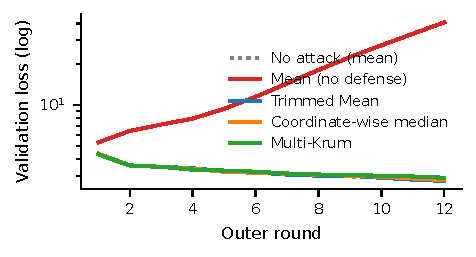
\includegraphics[width=\columnwidth]{figures/eval_byzantine.pdf}
\caption{10 workers, 3 adversarial (30\%), sign-flip attack, 12 outer rounds: undefended mean diverges; Trimmed Mean, Median, and Multi-Krum track the attack-free baseline.}
\label{fig:byzantine}
\end{figure}

A 10-worker cohort trains with 3 adversarial members (30\%, the design bound) mounting either a \emph{sign-flip} attack ($\Delta w \mapsto -5\Delta w$, a coordinated reversal and amplification of the true update) or a \emph{noise} attack (zero-mean Gaussian at $10\times$ honest magnitude). Table~\ref{tab:byz} and Fig.~\ref{fig:byzantine} summarize 12 outer rounds. Under sign-flip, undefended averaging diverges monotonically (40.7 and climbing, vs.\ attack-free 2.83); all three robust estimators finish at or below baseline (2.75--2.90). The zero-mean noise attack barely moves the mean---uncoordinated noise partially cancels across adversaries and rounds---illustrating why coordinated, directional attacks are the relevant threat. Sweeping the adversarial count for Trimmed Mean ($\beta{=}0.3$) under sign-flip locates the breakdown: $f/N \in \{10\%, 20\%, 30\%\}$ hold at baseline (2.87/2.84/2.75); $f/N = 40\%$---beyond the trim fraction---diverges (19.0), matching the $\alpha \le \beta$ tolerance predicted by Yin et al.~\cite{yin2018byzantine}.

\begin{table}[t]
\caption{Final validation loss after 12 outer rounds (10 workers, 30\% adversarial unless noted)}
\label{tab:byz}
\centering
\begin{tabular}{@{}lcc@{}}
\toprule
\textbf{Aggregation} & \textbf{Sign-flip} & \textbf{Noise} \\
\midrule
No attack (mean) & \multicolumn{2}{c}{2.83} \\
\midrule
Mean (no defense) & 40.67 & 2.52 \\
Trimmed Mean ($\beta{=}0.3$)~\cite{yin2018byzantine} & 2.75 & 2.82 \\
Coordinate-wise Median~\cite{yin2018byzantine} & 2.79 & 2.84 \\
Multi-Krum~\cite{blanchard2017machine} & 2.90 & 2.90 \\
\midrule
Trimmed Mean, $f{=}10\%$ / $20\%$ & 2.87 / 2.84 & --- \\
Trimmed Mean, $f{=}40\%$ (beyond bound) & 19.04 & --- \\
\bottomrule
\end{tabular}
\end{table}

\subsection{Compression Fidelity}
\label{sec:eval-compression}

Applying the repo compressor to real pseudo-gradients (0.62M-parameter model, 50-step deltas): Top-$K{=}5\%$/$10\%$/$20\%$ with int8 quantization and zlib yields $20.6\times$/$10.8\times$/$5.6\times$ size reduction at cosine fidelity 0.46/0.58/0.73. Fidelity alone understates usefulness: discarded mass is not lost---error feedback re-injects it in later rounds, giving the converging compressed trajectory of Fig.~\ref{fig:convergence}. We accordingly report the default pipeline as its \emph{measured} ${\sim}11\times$ payload compression, rather than a figure that conflates compression with sparsity ratios.

\subsection{PoNW Overheads}
\label{sec:eval-ponw}

A cohort-sync proof serializes to 763 bytes---${\sim}3{,}300\times$ smaller than the 2.5\,MB pseudo-gradient it attests. Signing costs 1.5\,ms, verification 0.56\,ms (pure-Python secp256k1; accelerated libraries cut this substantially). Challenge re-computation of one claimed step costs ${\sim}97$\,ms on our testbed---almost exactly the prover's own per-step cost on the same hardware, the intended cost symmetry of PoL-style verification. At the large-network spot-check floor (Section~\ref{sec:adaptive}), expected verification overhead is 5\% of network compute.

\subsection{Fault Tolerance under Churn}
\label{sec:eval-churn}

We deploy three containerized nodes (tiny model, Docker LAN, local tracker) and inject failures. Killing one node at $t{=}123$\,s of a 5-minute run, the survivors advance monotonically ($642 \to 2070$ aggregate steps) with no crash and continued loss descent. In a 10-minute run with kill at $t{=}180$\,s and restart at $t{=}275$\,s, the restarted node rejoins via tracker/DHT, resumes training (583 post-restart steps), and re-converges (loss 0.19 vs.\ 0.04 for uninterrupted peers, still descending); all nodes finish healthy, all gate thresholds pass. A 15-minute steady-state run sustains 4{,}721 aggregate steps with zero crashes. These LAN gates validate crash/rejoin machinery, complementing WAN-scale fault-tolerance evidence from~\cite{jaghouar2024intellect,ryabinin2023swarm}.

\section{Discussion}

\subsection{Scalability and Convergence}

The two-level hierarchy decouples intra-quorum traffic (high-frequency, speed-matched) from inter-quorum traffic (low-frequency outer syncs): aggregate throughput scales with the number of quorums, while per-node communication is governed by cohort size and cadence rather than network size. Two caveats: cohort gossip grows with replication factor, and the memory bound~\eqref{eq:budget} is necessary but not sufficient---activation-streaming bandwidth binds first for large models on consumer links. On convergence, DiLoCo-family methods match synchronous training at moderate $H$~\cite{douillard2023diloco,jaghouar2024opendiloco}, and our measurements agree (Fig.~\ref{fig:convergence}); but NeuroShard changes the aggregation operator, and robust estimators discard tail information that under non-i.i.d.\ shards need not be adversarial. Guarantees for Nesterov outer optimization composed with trimmed aggregation under heterogeneous data remain unproven; our evidence is empirical.

\subsection{Limitations and Future Work}
\label{sec:limitations}

Current limitations: (1)~evaluation is small-scale and CPU-bound---far from the design's target operating point, so 10B+-scale claims rest on the cited external systems, not our runs; (2)~PoNW's exact-replay defense weakens under cross-hardware floating-point non-determinism (Section~\ref{sec:ponw-spoofing}); (3)~the optimistic window imposes a 10-minute reward-finality floor; (4)~quorum bootstrapping requires layer-holder diversity; (5)~robust-aggregation guarantees under non-i.i.d.\ data are open. Future work, in priority order: a public testnet with GPU nodes on residential links, reporting utilization and convergence at $\geq$1B parameters against OpenDiLoCo/INTELLECT-1 baselines; simulation under realistic WAN latency/outage distributions and adversarial verifier behavior; TOPLOC-style non-determinism-robust commitments~\cite{ong2025toploc}; adaptive per-tier sync cadences; trusted-execution attestation; and formal convergence analysis. The prototype, harnesses, and raw results will be open-sourced with the camera-ready version.

\section{Conclusion}

NeuroShard extends low-communication decentralized LLM training into the open, adversarial, incentive-driven regime: speed-matched quorum pipelines, a DiLoCo-derived outer loop hardened with Byzantine-robust $\sqrt{n}$-weighted aggregation, and Proof of Neural Work tying rewards to re-executable evidence of training. Prototype experiments confirm the composed protocol's core behaviors---synchronous-quality convergence at orders-of-magnitude lower communication, resilience at the designed 30\% adversarial fraction with breakdown located empirically beyond it, sub-kilobyte proofs, and survival of node churn. The path from here is scale: from validated prototype to a public network able to stand beside its permissioned predecessors.

\bibliographystyle{IEEEtran}

\balance
\begin{thebibliography}{00}

\bibitem{openai2023gpt4}
OpenAI, ``GPT-4 technical report,'' \emph{arXiv:2303.08774 [cs.CL]}, Mar. 2023.

\bibitem{mcmahan2017communication}
B.~McMahan, E.~Moore, D.~Ramage, S.~Hampson, and B.~A.~y~Arcas, ``Communication-efficient learning of deep networks from decentralized data,'' in \emph{Proc.\ 20th Int.\ Conf.\ Artif.\ Intell.\ Statist.\ (AISTATS)}, Fort Lauderdale, FL, 2017, pp.~1273--1282.

\bibitem{kairouz2021advances}
P.~Kairouz \emph{et~al.}, ``Advances and open problems in federated learning,'' \emph{Found.\ Trends Mach.\ Learn.}, vol.~14, no.~1--2, pp.~1--210, 2021.

\bibitem{borzunov2023petals}
A.~Borzunov \emph{et~al.}, ``Petals: Collaborative inference and fine-tuning of large models,'' in \emph{Proc.\ 61st Annu.\ Meeting Assoc.\ Comput.\ Linguist.\ (ACL): System Demonstrations}, Toronto, Canada, 2023, pp.~38--44.

\bibitem{ryabinin2020hivemind}
M.~Ryabinin and A.~Gusev, ``Towards crowdsourced training of large neural networks using decentralized mixture-of-experts,'' in \emph{Adv.\ Neural Inf.\ Process.\ Syst.\ (NeurIPS)}, vol.~33, 2020, pp.~3659--3672.

\bibitem{douillard2023diloco}
A.~Douillard \emph{et~al.}, ``DiLoCo: Distributed low-communication training of language models,'' \emph{arXiv:2311.08105 [cs.LG]}, Nov. 2023.

\bibitem{jaghouar2024opendiloco}
S.~Jaghouar, J.~M.~Ong, and J.~Hagemann, ``OpenDiLoCo: An open-source framework for globally distributed low-communication training,'' \emph{arXiv:2407.07852 [cs.LG]}, Jul. 2024.

\bibitem{jaghouar2024intellect}
S.~Jaghouar \emph{et~al.}, ``INTELLECT-1 technical report,'' \emph{arXiv:2412.01152 [cs.DC]}, Dec. 2024.

\bibitem{sani2024photon}
L.~Sani \emph{et~al.}, ``Photon: Federated LLM pre-training,'' \emph{arXiv:2411.02908 [cs.LG]}, Nov. 2024.

\bibitem{ryabinin2023swarm}
M.~Ryabinin, T.~Dettmers, M.~Diskin, and A.~Borzunov, ``SWARM parallelism: Training large models can be surprisingly communication-efficient,'' in \emph{Proc.\ 40th Int.\ Conf.\ Mach.\ Learn.\ (ICML)}, vol.~202, Honolulu, HI, 2023, pp.~29416--29440.

\bibitem{warnat2021swarm}
S.~Warnat-Herresthal \emph{et~al.}, ``Swarm learning for decentralized and confidential clinical machine learning,'' \emph{Nature}, vol.~594, pp.~265--270, 2021.

\bibitem{maymounkov2002kademlia}
P.~Maymounkov and D.~Mazi\`{e}res, ``Kademlia: A peer-to-peer information system based on the XOR metric,'' in \emph{Proc.\ 1st Int.\ Workshop Peer-to-Peer Syst.\ (IPTPS)}, Cambridge, MA, Mar. 2002, pp.~53--65.

\bibitem{kaplan2020scaling}
J.~Kaplan, S.~McCandlish, T.~Henighan, T.~B.~Brown, B.~Chess, R.~Child, S.~Gray, A.~Radford, J.~Wu, and D.~Amodei, ``Scaling laws for neural language models,'' \emph{arXiv:2001.08361 [cs.LG]}, Jan. 2020.

\bibitem{hoffmann2022training}
J.~Hoffmann \emph{et~al.}, ``Training compute-optimal large language models,'' in \emph{Adv.\ Neural Inf.\ Process.\ Syst.\ (NeurIPS)}, vol.~35, 2022, pp.~30016--30030.

\bibitem{zhang2019root}
B.~Zhang and R.~Sennrich, ``Root mean square layer normalization,'' in \emph{Adv.\ Neural Inf.\ Process.\ Syst.\ (NeurIPS)}, vol.~32, 2019, pp.~12360--12371.

\bibitem{su2021roformer}
J.~Su, Y.~Lu, S.~Pan, A.~Murtadha, B.~Wen, and Y.~Liu, ``RoFormer: Enhanced transformer with rotary position embedding,'' \emph{arXiv:2104.09864 [cs.CL]}, Apr. 2021.

\bibitem{ainslie2023gqa}
J.~Ainslie, J.~Lee-Thorp, M.~de~Jong, Y.~Zemlyanskiy, F.~Lebr\'{o}n, and S.~Sanghai, ``GQA: Training generalized multi-query transformer models from multi-head checkpoints,'' in \emph{Proc.\ 2023 Conf.\ Empirical Methods Natural Lang.\ Process.\ (EMNLP)}, Singapore, 2023, pp.~4895--4901.

\bibitem{shazeer2020glu}
N.~Shazeer, ``GLU variants improve transformer,'' \emph{arXiv:2002.05202 [cs.LG]}, Feb. 2020.

\bibitem{blanchard2017machine}
P.~Blanchard, E.~M.~El~Mhamdi, R.~Guerraoui, and J.~Stainer, ``Machine learning with adversaries: Byzantine tolerant gradient descent,'' in \emph{Adv.\ Neural Inf.\ Process.\ Syst.\ (NeurIPS)}, vol.~30, 2017, pp.~118--128.

\bibitem{yin2018byzantine}
D.~Yin, Y.~Chen, K.~Ramchandran, and P.~Bartlett, ``Byzantine-robust distributed learning: Towards optimal statistical rates,'' in \emph{Proc.\ 35th Int.\ Conf.\ Mach.\ Learn.\ (ICML)}, vol.~80, Stockholm, Sweden, 2018, pp.~5650--5659.

\bibitem{jia2021proof}
H.~Jia \emph{et~al.}, ``Proof-of-learning: Definitions and practice,'' in \emph{Proc.\ 42nd IEEE Symp.\ Security Privacy (S\&P)}, San Francisco, CA, 2021, pp.~1039--1056.

\bibitem{zhang2022adversarial}
R.~Zhang \emph{et~al.}, ```Adversarial examples' for proof-of-learning,'' in \emph{Proc.\ 43rd IEEE Symp.\ Security Privacy (S\&P)}, San Francisco, CA, 2022, pp.~1408--1422.

\bibitem{fang2023proof}
C.~Fang \emph{et~al.}, ``Proof-of-learning is currently more broken than you think,'' in \emph{Proc.\ 8th IEEE Eur.\ Symp.\ Security Privacy (EuroS\&P)}, Delft, Netherlands, 2023, pp.~797--816.

\bibitem{ong2025toploc}
J.~M.~Ong \emph{et~al.}, ``TOPLOC: A locality sensitive hashing scheme for trustless verifiable inference,'' \emph{arXiv:2501.16007 [cs.CR]}, Jan. 2025.

\bibitem{primeintellect2025intellect2}
Prime Intellect Team, ``INTELLECT-2: A reasoning model trained through globally decentralized reinforcement learning,'' \emph{arXiv:2505.07291 [cs.LG]}, May 2025.

\bibitem{kalodner2018arbitrum}
H.~Kalodner, S.~Goldfeder, X.~Chen, S.~M.~Weinberg, and E.~W.~Felten, ``Arbitrum: Scalable, private smart contracts,'' in \emph{Proc.\ 27th USENIX Security Symp.}, Baltimore, MD, Aug. 2018, pp.~1353--1370.

\bibitem{bittensor}
Y.~Const and J.~Fishman, ``Bittensor: A peer-to-peer intelligence market,'' \emph{Bittensor Whitepaper}, 2022. [Online]. Available: \url{https://bittensor.com/whitepaper}

\bibitem{gensyn}
Gensyn, ``Gensyn technical paper,'' 2023. [Online]. Available: \url{https://docs.gensyn.ai}

\bibitem{karimireddy2020scaffold}
S.~P.~Karimireddy \emph{et~al.}, ``SCAFFOLD: Stochastic controlled averaging for federated learning,'' in \emph{Proc.\ 37th Int.\ Conf.\ Mach.\ Learn.\ (ICML)}, vol.~119, 2020, pp.~5132--5143.

\bibitem{goyal2017accurate}
P.~Goyal \emph{et~al.}, ``Accurate, large minibatch SGD: Training ImageNet in 1 hour,'' \emph{arXiv:1706.02677 [cs.CV]}, Jun. 2017.

\bibitem{stich2019local}
S.~U.~Stich, ``Local SGD converges fast and communicates little,'' in \emph{Proc.\ 7th Int.\ Conf.\ Learn.\ Represent.\ (ICLR)}, New Orleans, LA, 2019.

\bibitem{huang2019gpipe}
Y.~Huang \emph{et~al.}, ``GPipe: Efficient training of giant neural networks using pipeline parallelism,'' in \emph{Adv.\ Neural Inf.\ Process.\ Syst.\ (NeurIPS)}, vol.~32, 2019, pp.~103--112.

\bibitem{lin2018deep}
Y.~Lin, S.~Han, H.~Mao, Y.~Wang, and W.~J.~Dally, ``Deep gradient compression: Reducing the communication bandwidth for distributed training,'' in \emph{Proc.\ 6th Int.\ Conf.\ Learn.\ Represent.\ (ICLR)}, Vancouver, Canada, 2018.

\bibitem{alistarh2017qsgd}
D.~Alistarh, D.~Grubic, J.~Li, R.~Tomioka, and M.~Vojnovic, ``QSGD: Communication-efficient SGD via gradient quantization and encoding,'' in \emph{Adv.\ Neural Inf.\ Process.\ Syst.\ (NeurIPS)}, vol.~30, 2017, pp.~1709--1720.

\bibitem{karimireddy2019error}
S.~P.~Karimireddy, Q.~Rebjock, S.~U.~Stich, and M.~Jaggi, ``Error feedback fixes SignSGD and other gradient compression schemes,'' in \emph{Proc.\ 36th Int.\ Conf.\ Mach.\ Learn.\ (ICML)}, 2019, pp.~3252--3261.

\bibitem{vassilev2024adversarial}
A.~Vassilev, A.~Oprea, A.~Fordyce, and H.~Anderson, ``Adversarial machine learning: A taxonomy and terminology of attacks and mitigations,'' NIST Rep.\ AI 100-2e2023, 2024.

\end{thebibliography}

\end{document}
